\chapter{Homology}
Before going into what \textit{persistent} homology is, it is well worth our time clearly stating what we mean by homology. Broadly speaking, homology is an invariant of topological spaces concerned with cycles in the space that are not boundaries. More abstractly, homology captures the notion of ``$n$-dimensional holes'' in the space.

In \textit{persistent} homology we generally work without predefined topological spaces and start with a basic data set which, at best, has some metric structure that we can use to endow it with some type of complex. The main complex we will be working on is the simplicial complex, since computationally we can approximate such a complex on a set of data points. We will also review homology of cubical complexes related to one of the case studies in Chapter 4. Therefore the classical definitions involving concepts such as singular homology are not something we will dwell on, but instead we refer the reader to Hatcher's excellent exposition in \cite{hatcher2002}.


\section{Simplices}
We start with what will constitute our atoms in simplicial homology, namely the simplices.
\begin{definition}[{\cite[p. ~62]{edels}}]
  An \textbf{$n$-simplex} is the convex hull in $\mathbb{R}^{m}$ of $n+1$  points $v_{0},\dots,v_{n}$ such that the vectors $v_{1}-v_{0}, \dots, v_{n} - v_{0}$ are linearly independent. The points $v_{0},\dots,v_{n}$ are known as the \textbf{vertices} of the simplex. The number $n$ is the \textbf{dimension} of a simplex.
\end{definition}

The positions of a simplex vertices in Euclidean space are not very important in a topological sense: a bijection between two simplices' vertex sets induces a canonical homeomorphism between the two simplices.

As seen in Figure \ref{simplices} the $0,1,2$ and $3$-dimensional simplices are familiar shapes consisting of vertices, edges, triangles and tetrahedrons.

\begin{figure}
  \centering
  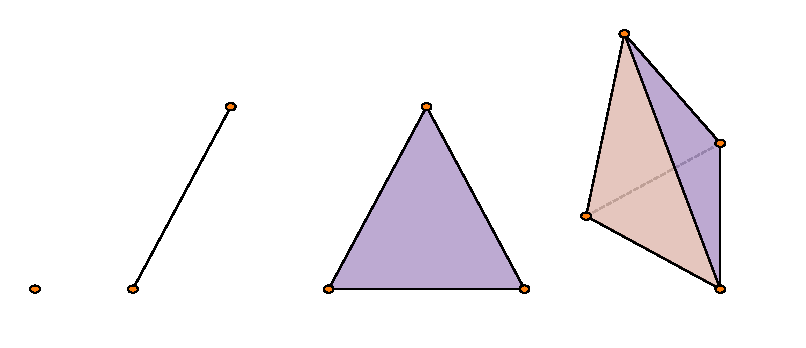
\includegraphics[]{simplex.pdf}
  \caption{
  \label{simplices}
0-simplex (left), 1-simplex (middle left), 2-simplex (middle right) and 3-simplex (right).}
  \end{figure}
\begin{definition}[{\cite[p. ~62]{edels}}]
A \textbf{face} of a simplex is the convex hull of a subset of its vertices. If $\tau$ is a face of $\sigma$ we write $\tau \subset \sigma$.
\end{definition}
% Since higher dimensional simplices are formed by simplices of lower dimensions we can always decompose a simplex into its faces. For example, a 2-simplex can be decomposed into the three edges that make up the triangle.
%
% Since the boundary of a simplex is formed by simplices of oneowdimension l, we can always decompose a simplex into its collection of faces. For example, a 2-simplex can be decomposed into the three edges that form a triangle, the boundary of a 2-simplex.
Note that the boundary of a simplex can be decomposed as a union of faces of one dimension lower than the simplex itself. For example, the boundary of a 2-simplex is the union of the three edges that surround the interior of the triangle.
\section{Simplicial Complex}
By gluing together simplices at their faces as seen in Figure \ref{complex2} we can construct higher-order objects, which we call simplicial complexes.

\begin{definition}[{\cite[p. ~63]{edels}}] \label{defsimcomp}
A (finite) \textbf{simplicial complex} $K$ is a finite collection of simplices such that

\begin{itemize}
    \item $\sigma \in K$ and $\tau \subset \sigma$ implies that $\tau \in K$,
    \item $\sigma_{1}, \sigma_{2} \in K$ implies that $\sigma_{1} \cap \sigma_{2}$ is either empty or a face of both.
\end{itemize}
The \textbf{dimension} of the simplicial complex $\dim(K)$ is the largest dimension of any simplex in the complex.
\end{definition}

\begin{figure}
  \centering
  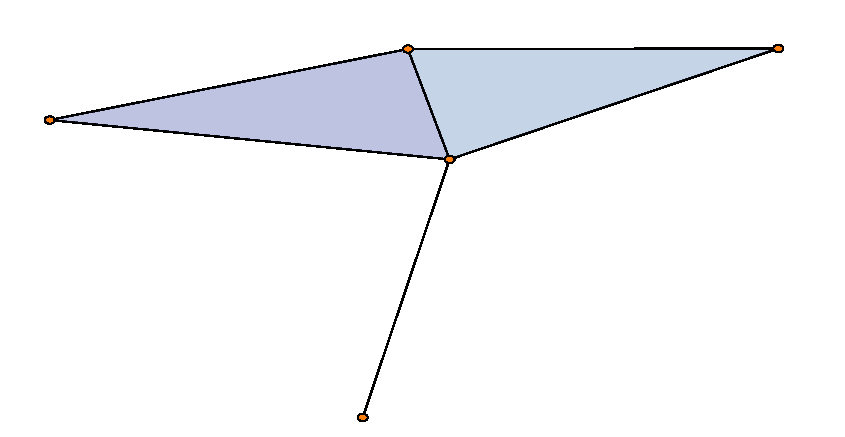
\includegraphics[scale=0.7]{complex.pdf}
  \caption{ \label{complex2} Example of a simplicial complex consisting of two 2-simplices glued together with an attached 1-simplex.}
\end{figure}

The first requirement in the definition tells us that a simplicial complex contains the faces of all its simplices. The second requirement tells us that the simplices are only glued together at shared faces.

It is possible to consider simplicial complexes which allow for an infinite number of simplices, however for our purposes it is sufficient to only consider \textit{finite} simplicial complexes. Hence, when we say ``simplicial complex'' it is to be understood as ``finite simplical complex'' in the sense of Definition \ref{defsimcomp}.


We will refer to the construction in Definition \ref{defsimcomp} as a \textbf{geometric simplicial complex}. This is to distinguish the geometric simplicial complex from a simplicial complex where we discard the geometric connotations. It is possible to define a combinatorial simplicial complex by only considering the set of the vertices for each simplex.

\begin{definition}[{\cite[p. ~62]{edels}}]  \label{defabstractsimcomp}
An \textbf{abstract simplicial complex} $K$ is a finite collection of sets such that $\alpha \in K$ and $\beta \subseteq \alpha$ implies that $\beta \in K$.
\end{definition}

This abstract definition coincides with the geometric definition by calling the elements of $K$ its simplices. The simplices of $K$ are no longer geometric objects in Euclidean space, but simply combinatorial objects consisting of vertex sets.

\begin{definition}
Given a geometric simplicial complex $K$, we can construct an abstract simplicial complex $A$ by translating each simplex $\sigma_{i} \in K$ to a set $\{v_{0},\dots,v_{n}\}$ where each $v_{i}$  denotes the presence of a vertex. We call $K$ a \textbf{geometric realization} of $A$.
\end{definition}
Hence, we can always transition from a geometric simplicial complex to an abstract simplicial complex. There is an elementary result that allows the construction in the other direction.
\begin{theorem}[{\cite[Geometric Realization Theorem, p. ~64]{edels}}]\label{geometricthm}
Every abstract simplicial complex of dimension $n$ has a geometric realization in $\mathbb{R}^{2n+1}$.
\end{theorem}
While there are many different possible geometric realizations for a given abstract simplicial complex, any two realizations of the same abstract simplicial complex are homeomorphic \cite[Theorem 3.1, p. ~15]{munkres}. Hence, Theorem \ref{geometricthm} guarantees the existence of a geometric realization unique up to topological equivalence.

It is helpful to be able to talk about a specific face of a simplex, but to do so we need some notion of order between the vertices. This motivates the following definition.
\begin{definition} \label{defordsimcomp}
An \textbf{ordered} simplicial complex $K$ is an abstract simplicial complex together with a partial order on the set of vertices of $K$, which restricts to a total order on each simplex.
\end{definition}
The restriction of the partial order on the vertices to a total order on  $\sigma$ means that $\sigma$ can be seen as an ordered set $[v_{0},\dots,v_{n}]$. Therefore, the notion of the $i$th face of $\sigma$ is well-defined and is given by $[v_{0},\dots,\hat v_{i},\dots,v_{n}]$ where $\hat v_{i}$ denotes the exclusion of this particular vertex.

Note that by enumerating the vertices of an abstract simplicial complex we get a total order on its vertices, which turns any abstract simplicial complex into an ordered simplicial complex.

From here on we will refer to an ordered simplicial complex as a simplicial complex unless stated otherwise. This allows us to state our definitions and work with simplices solely as combinatorial objects.
\section{Simplicial Homology}
Roughly speaking, in topology when two spaces are homeomorphic, they share the same topological properties. One such property is the algebraic structure of the holes, voids and higher-dimensional equivalents in the space.
Homology can generally thought of as being the characterization of these holes in a topological space. Beyond that however, it is a way of associating algebraic objects to topological spaces. In the context of simplicial complexes, we first need some algebraic machinery to precisely define what we mean by holes in a simplicial complex.

\begin{definition}[\cite{Zomorodian2005}]\label{chainmodulesimp}
  The $k$th \textbf{chain module} $C_{k}(K)$ on a (ordered) simplicial complex $K$ is the free module with basis given by the $k$-dimensional simplices in $K$ with coefficients in some ring $R$ with additive unit $0$ and multiplicative unit $1$. In other words, the elements of $C_{k}(K)$ are formal sums
  \[ \sum_{i} r_{i}\sigma_{i}\]
  where $r_{i} \in R$ and $\sigma_{i}$ is a $k$-dimensional simplex in $K$. % Furthermore, there is an equivalence of elements in the chain module such that $\sigma = -\tau$ if $\tau$ is given by an odd permutation of the vertices of $\sigma$.
\end{definition}

% To see that the chain module $C_{k}(K)$ is still free under the relation note that

\begin{definition}[{\cite[p. ~2]{weibel1994}}]
  A \textbf{chain complex} $C_{*}$ over a ring $R$ is a family of $R$-modules $\{C_{k}\}_{k
  \in \mathbb{Z}}$ with $R$-module maps $\partial_{k}: C_{k} \to C_{k-1}$ such that the composition $\partial_{k-1} \circ \partial_{k}$ is the zero map. We call the maps $\partial_{k}$ the \textbf{differentials} of the chain complex.
\end{definition}

In other words, a chain complex is just a sequence of modules with maps between them such that the maps cannot carry an element further than one level below in the complex.
\begin{example}
  The sequence of $\mathbb{Z}$-modules
\begin{center}
\begin{tikzcd}
  \dots \arrow[]{r}{\partial_{k+1}} & \mathbb{Z} \arrow[]{r}{\partial_{k}} & \mathbb{Z} \arrow[]{r}{\partial_{k-1}} & \mathbb{Z} \arrow[]{r}{\partial_{k-2}} & \dots \arrow[]{r}{\partial_{1}} & \mathbb{Z} \arrow[]{r}{\partial_0} & \mathbb{Z}
\end{tikzcd}
\end{center}
with differentials
\[ \partial_{k}(n)
  \begin{cases} k \cdot n & \text{if }k \text{ is odd} \\
                0 & \text{if }k \text{ is even}
    \end{cases}
  \]
is a chain complex since the composition of any consecutive differentials $\partial_{k-1}\partial_{k}$ necessitates that either $k-1$ or $k$ is even, hence the composition has to be the zero map.
\end{example}

\begin{theorem}\label{simpchainthm}
Given a sequence $C_{*}$ of chain modules with coefficients in a ring $R$ on a simplicial complex $K$
\begin{center}
\begin{tikzcd}
  \dots \arrow[]{r}{\partial_{k+1}} & C_k(K) \arrow[]{r}{\partial_{k}} & C_{k-1}(K) \arrow[]{r}{\partial_{k-1}} & C_{k-2}(K) \arrow[]{r}{\partial_{k-2}} & \dots \arrow[]{r}{\partial_{1}} & C_0(K) \arrow[]{r}{\partial_0} & 0
\end{tikzcd}
\end{center}
where we define the differential $\partial_{k}$ as
\begin{align*}
& \partial_{k}:  C_{k}(K) \to C_{k-1}(K) \\
& \partial_{k}(\sigma) =  \sum^{k}_{{i=0}} (-1)^{i} [v_{0},\dots,\hat v_{i}, \dots, v_{k}]
\end{align*}
Then $C_{*}$ is a chain complex, or equivalently $\partial_{k-1}\partial_{k}=0$ for all $k$.
\end{theorem}

\begin{proof}
  We drop the subscripts on the differentials for convenience, so what we need to show becomes $\partial \partial \sigma = 0 $ for any simplex $\sigma$. Since $\partial$ is a homomorphism the result extends to arbitrary chains in the chain module in which $\sigma$ lives. By linearity of a homomorphism we get
  \begin{align*}
    \partial \partial \sigma =& \sum_{i} (-1)^{i} \partial [v_{0}, \dots, \hat v_{i}, \dots v_{n}] \\
    =& \sum_{j < i} (-1)^{i} (-1)^{j} [ \dots,  \hat v_{j}, \dots , \hat v_{i}, \dots ] \\ &+ \sum_{i < j} (-1)^{i} (-1)^{j-1}  [ \dots,  \hat v_{i}, \dots , \hat v_{j}, \dots ] \\
    =& 0.
  \end{align*}
  The first sum comes from when $j<i$ since when removing $v_{i}$ the position of $v_{j}$ is unchanged in the resulting simplex, whereas the second sum comes from the other possible case where $i<j$ and so removing $v_{i}$ causes the position of $v_{j}$ to shift by one. Hence, the sums cancel out and so $\partial \partial = 0$. \end{proof}
Note that the differential $\partial$ on a simplicial chain module is well-defined since the presence of a simplex in an ordered simplicial complex in which the notion of the $i$th face of simplex is well-defined.
\begin{example}
Given a simplicial complex $K$ consisting of a triangle without interior as in Figure \ref{trichain}, a chain in $C_{1}(K)$ would be a linear combination of edges. For example, an element of $C_{1}(K)$ is $[v_{0},v_{1}]+[v_{1},v_{2}]$ which is highlighted in green.
\begin{figure}[ht]
  \centering
  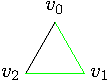
\includegraphics[scale=2]{trichain.pdf}
  \caption{\label{trichain} A simplicial complex in which the 1-chain $[v_{0},v_{1}]+[v_{1},v_{2}]$ is highlighted in green.}
\end{figure}
\end{example}

\begin{example}
  Consider the chain complex on the simplicial complex given by the $2$-simplex in Figure \ref{2simplex}.
\begin{center}
\begin{tabular}{*3l}
  Module & Generators \\ \midrule
  $C_{0}$ & $[v_{0}],[v_{1}],[v_{2}]$ \\
  $C_{1}$ & $[v_{0},v_{1}],[v_{1},v_{2}],[v_{0},v_{2}]$ \\
  $C_{2}$ & $[v_{0},v_{1},v_{2}]$
\end{tabular}
\end{center}
Then the differential on the sole generator of $C_{2}$ is given by
\[\partial_{2}([v_{0},v_{1},v_{2}])=[v_{1},v_{2}]-[v_{0},v_{2}]+[v_{1},v_{2}]\]
which geometrically, as seen in Figure \ref{2simplex}, is the boundary of the simplex. For this reason we also refer to the differential of a chain complex as the \textbf{boundary map} or \textbf{boundary operator}.
\begin{figure}[ht]
  \centering
  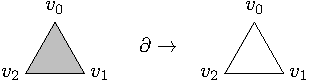
\includegraphics[scale=2]{partialtri.pdf}
  \caption{\label{2simplex} Illustration of how the differential maps a $2$-simplex to its boundary.}
\end{figure}
\end{example}
The notion of the differential being a map from a simplex to its boundary motivates the following definition.
\begin{definition}[{\cite[p. ~4]{weibel1994}}]
  Given a chain complex $C_{*}$ the \textbf{$k$-cycles} $Z_{k}$  and the \textbf{$k$-boundaries} $B_{k}$ of $K$ are the $R$-modules
  \[ Z_{k} := \ker \partial_{k}\]
  \[ B_{k} := \textrm{im } \partial_{k+1}.\]
  Just as for a chain complex we will sometimes refer to the collection of $Z_{k}$ and $B_{k}$ as $Z_{*}$ or $B_{*}$ respectively.
\end{definition}
Our overarching goal is to characterize $k$-cycles modulo $k$-boundaries. Hence, a vital result is this corollary to Theorem \ref{simpchainthm}.

\begin{corollary} \label{submodulecycle}
  The $k$-boundaries are a submodule of the $k$-cycles.
\end{corollary}


\begin{proof}
Let $\sigma \in B_{k} = \textrm{im } \partial_{k+1}$ then for some $\tau \in C_{k+1}$ we have that $\partial_{k+1}(\tau)=\sigma$. Hence,
\[ \partial_{k}(\sigma) = \partial_{k} \partial_{k+1}(\tau) = (\partial_{k} \circ \partial_{k+1}) \tau = 0\]
and so $\sigma \in \ker \partial_{k} = Z_{k}$.
\end{proof}

 Corollary \ref{submodulecycle} tells us that if we can find the cycles and ignore those which are just boundaries, then we have identified the holes. This motivates the following definition of homology.
\begin{definition}
  Given a simplicial chain complex \hspace{0.05cm}$C_{*}$ the homology module $H_{k}$ is defined as
  \[H_{k}(K) := Z_{k} / B_{k} = \ker(\partial_{k})/\text{im}(\partial_{k+1})\]
\end{definition}
Hence, the $k$th homology group captures precisely those cycles which are not in the image of the higher dimensional differential. In other words, the non-trivial equivalence classes represent the cycles which are not boundaries.
\begin{example}
Consider the chain complex over $\mathbb{Z}_{2}$ resulting from the simplicial complex in Figure \ref{trihom}.
\begin{figure}[ht]
  \centering
  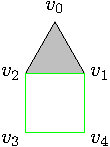
\includegraphics[scale=2]{trisquarefilled.pdf}
  \caption{\label{trihom} Illustration of a simplicial complex with a 1-cycle in green consisting of a square without interior.}
\end{figure}
There are two 1-cycles, the boundary of the filled triangle and the square. Since the boundary of the filled triangle is in $\text{im} (\partial_{2})$ we get that this element belongs to the trivial class in $H_{1}$. However, there is one non-trivial element given by the square without interior. So $H_{1}$ contains one non-trivial element generated by the cycle in green.

To quantify the number of linearly independent generators in a homology module $H_{k}$ we say that the \textbf{$k$th Betti number} is denoted $\beta_{k}$ where $\beta_{k} = \text{rank }(H_{k})$, the maximum number of linearily independent elements of $H_{k}$ as a module.

\section{Cubical Homology}
The definition of a chain complex is general enough that we need not limit ourselves to chain complexes arising from simplicial complexes. Since homology was defined on chain complex, regardless of how the chain complex was constructed, we get a well-defined notion of homology for free. Another type of complex which we can define chain complexes on are cubical complexes. As the atoms of simplicial complexes are simplices, the atoms of cubical complexes are cubes.

\begin{definition}[{\cite[Definition 2.1, p. ~40]{kaczynski2004}}]
An elementary interval is a unit interval $[k,k+1]$ or a degenerate interval $[k,k]$ for $k \in \mathbb{N}$.
\end{definition}

\begin{definition}[{\cite[Definition 2.3-2.4, p. ~40]{kaczynski2004}}]
  An \textbf{elementary cube} $Q$ is the Cartesian product of $n$ elementary intervals
  \[Q = \prod^{n}_{i=0} I_{i} \subset \mathbb{R}^{n}\]
  and where $n$ is known as the \textbf{embedding number} $emb(Q)$.
\end{definition}

\begin{definition}[{\cite[Definition 2.4, p. ~41]{kaczynski2004}}]
The \textbf{dimension} $dim(Q)$ of an elementary cube $Q$ is the number of non-degenerate intervals in the product of elementary intervals that make up $Q$.
\end{definition}

Under this definition a degenerate elementary interval is a $0$-dimensional cube and a non-degenerate elementary interval is a $1$-dimensional cube, which corresponds to our notion of vertices and edges in simplicial complexes.

We let $\mathcal{K}^{n}$ denote the set of all elementary cubes in $\mathbb{R}^{n}$. The set of all possible elementary cubes is then denote $\mathcal{K}$ defined as
\[ \mathcal{K}:= \bigcup^{\infty}_{n=1} \mathcal{K}^{n} \]
Additionally, we define
\[ \mathcal{K}_{k} := \{ Q \in \mathcal{K} \mid \dim Q = k \}\]
\[ \mathcal{K}^{n}_{k} := \{ \mathcal{K}_{k} \cap \mathcal{K}^{n} \}\]
where it is important to note that $K_{d} \neq K^{d}$ since $K^{d}$ contains any elementary cube embedded in $\mathbb{R}^{d}$. For instance $Q:=[0,0] \times [1,1] \times [2,2] \in \mathcal{K}^{3}$, but $Q \not \in K_{3}$ since $Q$ only consists of degenerate intervals and so $\dim Q = 0$.


\begin{definition}[{\cite[Definition 2.9, p. ~43]{kaczynski2004}}]
  A cubical set $X$ is a finite union of elementary cubes. Given a cubical set $X$ a cubical complex $\mathcal{K}(X)$ is defined as
  \[ \mathcal{K}(X):= \{Q \in \mathcal{K} \mid Q \subset X\}.\]
  Additionally we define the $k$-skeleton of the cubical complex as
  \[ \mathcal{K}_{k}(X):= \{ Q \in \mathcal{K}(X) \mid \dim Q = k \}.\]
\end{definition}

Much like in the case with the simplicial complexes, working with the actual geometric objects can be unwieldy when doing algebraic calculations. For this reason we introduce an abstract object for each elementary cube, called an elementary chain.
\begin{definition}[{\cite[p. ~48]{kaczynski2004}}]
  Given a cube $Q \in \mathcal{K}^{n}_{k}$ the elementary $k$-chain $\hat Q$ is a map
  \[\hat Q: \mathcal{K}^{n}_{k} \to \mathbb{Z}\]
\end{definition}

Furthermore, since elementary cubes consist of finite cartesian products of elementary intervals, we need a corresponding notion on elementary chains.

\begin{definition}[{\cite[Definition 2.23, p. ~51]{kaczynski2004}}]
Given two elementary cubes $P,Q$ the \textbf{cubical product} of the corresponding elementary $k$-chains $\hat P, \hat Q$ is defined as \[\hat P \diamond \hat Q:= \widehat{P \times Q}\]
\end{definition}
If we now fix some ring $R$ with additive unit $0$ and multiplicative unit $1$ we can proceed as for the simplicial case.
\begin{definition}[{\cite[Definition 2.27, p. ~53]{kaczynski2004}}]
  The \textbf{$k$th chain module} of a cubical complex $\mathcal{K}(X)$ is the free $R$-module $C_{k}(\mathcal{K}(X))$ whose elements are formal sums
  \[ \sum_{i} \alpha_{i} \hat Q_{i}\]
  known as \textbf{$k$-chains} where $\alpha_{i} \in R$ and $Q_{i} \in \mathcal{K}_{k}(X)$.
\end{definition}

The cubical product extends to $k$-chains in the following way.

\begin{definition}
The cubical product $\diamond$ of two $k$-chains $c_{1},c_{2}$ of a chain module on a cubical complex is \[ c_{1} \diamond c_{2} = \sum_{i} \sum_{j} \alpha_{i} \beta_{j} \hat P_{i} \diamond  \hat Q_{j}\]
\end{definition}

It can be shown with relative ease that the cubical product on $k$-chains is distributive, associative and to 0 if one of its arguments is 0, see \cite[Proposition 2.25, p. ~51]{kaczynski2004}.

All we need to do in order for the machinery of homology to be applicable is to define a boundary operator on the elements of the chain modules of a cubical complex which has the property that $\partial \partial = 0$.
\begin{definition}[{\cite[Definition 2.31, p. ~54]{kaczynski2004}}]
  The boundary map of an elementary cube is defined inductively on the embedding number cube in the following way. Let $Q$ be an elementary cube, we then have that
  \[ \partial \hat Q =
    \begin{cases}
      0 & Q = [k,k] \\
      \widehat{[k+1,k+1]} - \widehat{[k,k]} & Q = [k,k+1] \\
      \partial \hat I \diamond \hat P +(-1)^{\dim \hat I} \hat I \diamond \partial \hat P & Q=I \times P, emb(Q) \geq 2
    \end{cases}
  \]
  which extends linearly on $k$-chains.
\end{definition}
\begin{theorem}[{\cite[Proposition 2.37, p. ~58]{kaczynski2004}}]
The composed boundary map $\partial \partial$ is the zero map.
\end{theorem}
\begin{proof}
  Let $Q$ be an elementary cube. If $emb(Q)=0$ then by the definition of the boundary map $\partial (\partial Q) = \partial(0) = 0$. If $emb(Q)=1$ then
  \begin{align*}
    \partial \partial Q =& \partial([k+1,k+1]-[k,k]) \\ =&\partial([k+1,k+1])-\partial([k,k])
                                                          \\=&0-0\\=&0
  \end{align*}
We prove it for higher embedding numbers by induction. Assume it holds for $emb(Q)=n$, we want to prove that it also holds for $emb(Q)=n+1$.
\begin{align*}
  \partial \partial Q =& \partial(\partial \hat I \diamond \hat P) + \partial((-1)^{\dim I} \hat I \diamond \partial \hat P)
\end{align*}
Now assume that $\dim I = 0$ then $I$ is a degenerate interval and so we get
\begin{align*}
  \partial \partial Q =& \partial(0 \diamond \hat P) + \partial((-1)^{0} \hat I \diamond \partial \hat P) \\
  =& 0 + \partial( \hat I \diamond \partial \hat P) \\
  =& (\partial \hat I \diamond \partial \hat P + (-1)^{\dim I} \hat I \circ \partial \partial \hat P \\
  =& 0 + \hat I \diamond \partial \partial \hat P \\
  =& 0 + 0 \\
  =& 0
\end{align*}
where $\partial \partial \hat P = 0$ follows from the induction hypothesis since $\dim \hat P = n+1-1=n$. Now, let us assume the other case, namely that $\dim I = 1$ then we get
\begin{align*}
\partial \partial Q =& \partial(\partial \hat I \diamond \hat P) - \partial( \hat I \diamond \partial \hat P)\\
=& \partial \partial \hat I \diamond \hat P + (-1)^{\dim \partial I} \partial \hat I \diamond \partial \hat P - (\hat \partial I \diamond \partial \hat P - \hat I \diamond \partial \partial \hat P)\\
=& 0 + (-1)^{\dim \partial \hat I} \partial \hat I \diamond \partial \hat P - (\hat \partial I \diamond \partial \hat P - 0)\\
  =& \partial \hat I \diamond \partial \hat P - \partial \hat I \diamond \partial \hat P\\
  =& 0
\end{align*}
where $\dim \partial \hat I = 0$ since $ I$ is an elementary interval. Since we have now shown the induction hypothesis holds for $n+1$ given it holds for $n$, this concludes the proof by induction.
\end{proof}
We now have everything necessary to construct a chain complex on cubical complexes: a sequence of $R$-modules, the $k$-chain modules on cubical complexes, and module homomorphisms $\partial$ which have the property of $\partial \partial = 0$. Since our prior definitions with regards to \textit{homology} were entirely stated in terms of chain complexes we can be assured that homology on chain complexes given by cubical complexes is well-defined.

%%% Local Variables:
%%% mode: latex
%%% TeX-master: "thesis.tex"
%%% End:
